\section{Imaging and Image Processing}
At some point between a biological brain processing the life of an organism, and
a simulation of a brain attempting to continue computation, the brain must be
"copied" over. This can be done through several different imaging techniques.

\begin{figure}[h]
    \centering
    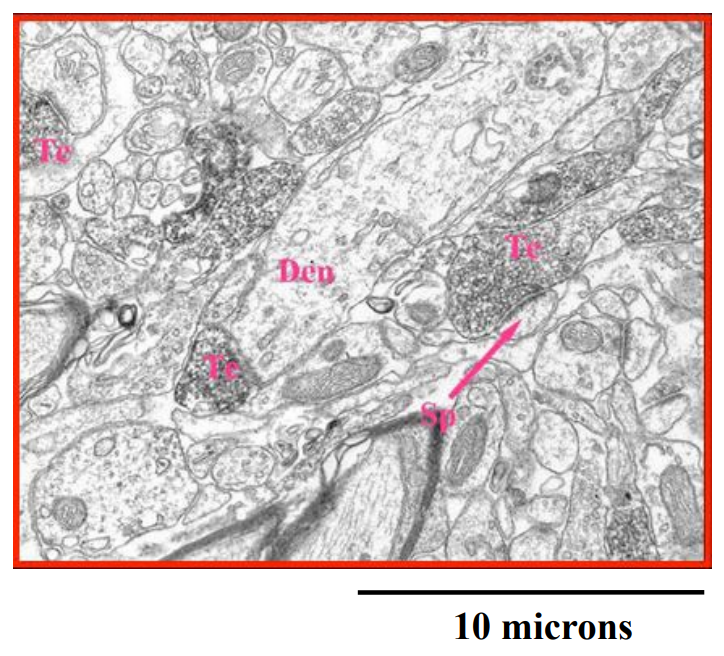
\includegraphics{figures/graphs/scaleexample.png}
    \DoubleCaption{scaleexample}
    {temp}
    \label{scaleexample}
\end{figure}
\vspace{1ex}

\subsection{Current Methods of Scanning the brain}

\subsubsection*{MRI Scanning}

- Common procedure
- Enough detail for general structure, but provides little to no insight to fine
details such as placement of dendritic!Typo?! spines or the exact size or placement of
synapses between neurons.
- As the patient is typically alive during a scan, there will be significant
measurement drift as the current is still moving around the brain as normal.

\subsubsection*{XRay}

- Not naturally useful, have to inject a substrate into the brain for this to
create an image of any meaningful contrast ?!?!CITE

\subsubsection*{Electron Microscope Scanning}

- Very precise
- Can take a very long time
- Need well "frozen" slices of the brain for this to be of any use or you'll
have major measurement drift as the brain decays.

\subsubsection*{New Methods}

- Some of the more experimental stuff here.

\subsection[Error induced through noise]{Examination of Error induced through the imaging process}

Prediction of future brain activity through simulation requires an accurate and
detailed connectome of a brain, with synapses and neurons correctly located in
space.\autocite{bostrom_whole_2008} The accuracy of such a model depends on the
resolution of the imaging method used to create it. The error resulting from
such a imaging method is the measurement error. Depending on imaging procedure, brain matter may shift in composition during the course of the scan, which is the cause of measurement drift, itself a form of measurement error.

\setlength{\tabcolsep}{4ex}
\renewcommand{\arraystretch}{1.1}
\begin{table}[ht]
    \centering
    \begin{tabular}{@{}llll@{}}
        Method              & Resolution                 & Time    & Error(approx.) \\
        \hline
        MRI                 & 6$\mu m$                   & 30mins  & 95\%           \\
        MRI microscopy      & 3$\mu m$                   & -       & 85\%           \\
        XRay microscopy     & 30nm                       & -       & 30\%           \\
        Electron microscopy & \textasciitilde 30nm-0.1nm & >3mnths & <1\%           \\
        Theoretical Ideal   & <5nm                       & <500s   & <1\%           \\
        \hline
    \end{tabular}
    \DoubleCaption{Comparison of imaging methods.}{Error approximated from size of dendritic spines.}
    \label{imagemethodcomparison1}
\end{table}
\setlength{\tabcolsep}{1ex}

\subsubsection[Error induced through low resolution]{Effect of Low Resolution} 
(this is easy just print something out
and scan it badly. Explain what kind of error in incurred.)